\documentclass[oneside, mag]{mgr}	
 
\usepackage{polski}	
\usepackage[utf8]{inputenc}	
\usepackage{amsmath}		
\usepackage{graphicx}	
\graphicspath{ {./} }
\usepackage{amsfonts}
\usepackage{hyperref}
\usepackage{tabstackengine}
\usepackage{caption}
\usepackage{subfig}
\usepackage{listings}

\newcommand{\bb}{\textbf}

\title{Analiza efektywności zastosowania sieci rekurencyjnych w zadaniu klasyfikacji}	
\engtitle{Analysis of the effectiveness of recursive networks in the classification task}
\author{Jędrzej Kozal}
\supervisor{dr  inż. Paweł Ksieniewicz}

\field{Informatyka (Inf)}
\specialisation{Systemy informatyki w medycynie (IMT)}

\begin{document}
\bibliographystyle{plabbrv}	

\maketitle

\chapter{Wstęp}

\section{Wprowadzenie}

\cite{Goodfellow-et-al-2016}

\section{Przegląd literatury}

Sieci Rekurencyjne zostały oparte na pracy Rumelharta \cite{RNN}. Algorytm uczenia RNN - propagacja wsteczna w czasie (Back-Propagation Through Time - BPTT) zostały przedstawione w \cite{BPTT}.
Udowodniono, że przy pewnych założeniach RNN mogą być kompletne w sensie Turinga \cite{turing-complete}.
Wprowadzono wiele modyfikacji w zasadach działania i strukturze RNN. W \cite{bidirectional} wprowadzono sieci dwukierunkowe, przetwarzające sekwencje w dwóch kierunkach: od początku do końca sekwencji i od końca do początku. Ostateczna wartość dla n-tego elementu sekwencji jest obliczana na podstawie n-tego wyniku dla obu kierunków.
RNN w swojej natywnej formie nie są w stanie nauczyć się długich zależności w ciągu uczącym. Problem ten jest w znacznej mierze spowodowany wybuchającymi lub znikającymi gradientami (exploding or vanishing gradients, \cite{vanishing_gradient_RNN}).

Sieci Rekurencyjne znalazły wiele zastosowań w przetwarzaniu sekwencji. (opisać zastosowania) NLP: tłumaczenie, modele języka, naśladowanie stylu, przetwarzanie dźwięków: generowanie mowy, generowanie muzyki, sentiment analysis 

Sieci rekurencyjne są także wykorzystywane w połączeniu z innymi modelami jak np. labelowanie imgages.

W \cite{DBLP:journals/corr/VisinKCMCB15} wykorzystano sieć rekurencyjną do klasyfikacji obrazów i porównano uzyskane wyniki z rezultatami dla sieci konwolucyjnych. Proponowany model (ReNet) wykorzystywał RNN do czterotnego trawersowania fragmentów obrazu w celu ekstrakcji cech, jako alternatywę dla warstw konwolucyjnych z poolingiem. W \cite{DBLP:journals/corr/KalchbrennerDG15} przedstawiono GRID LSTM, które rozszerzało standardowy model sieci LSTM do N-wymiarowych komórek ze współdzielonymi wektorami stanu i pamięci.

\chapter{Omówienie wybranych metod}

\begin{figure}
\centering
	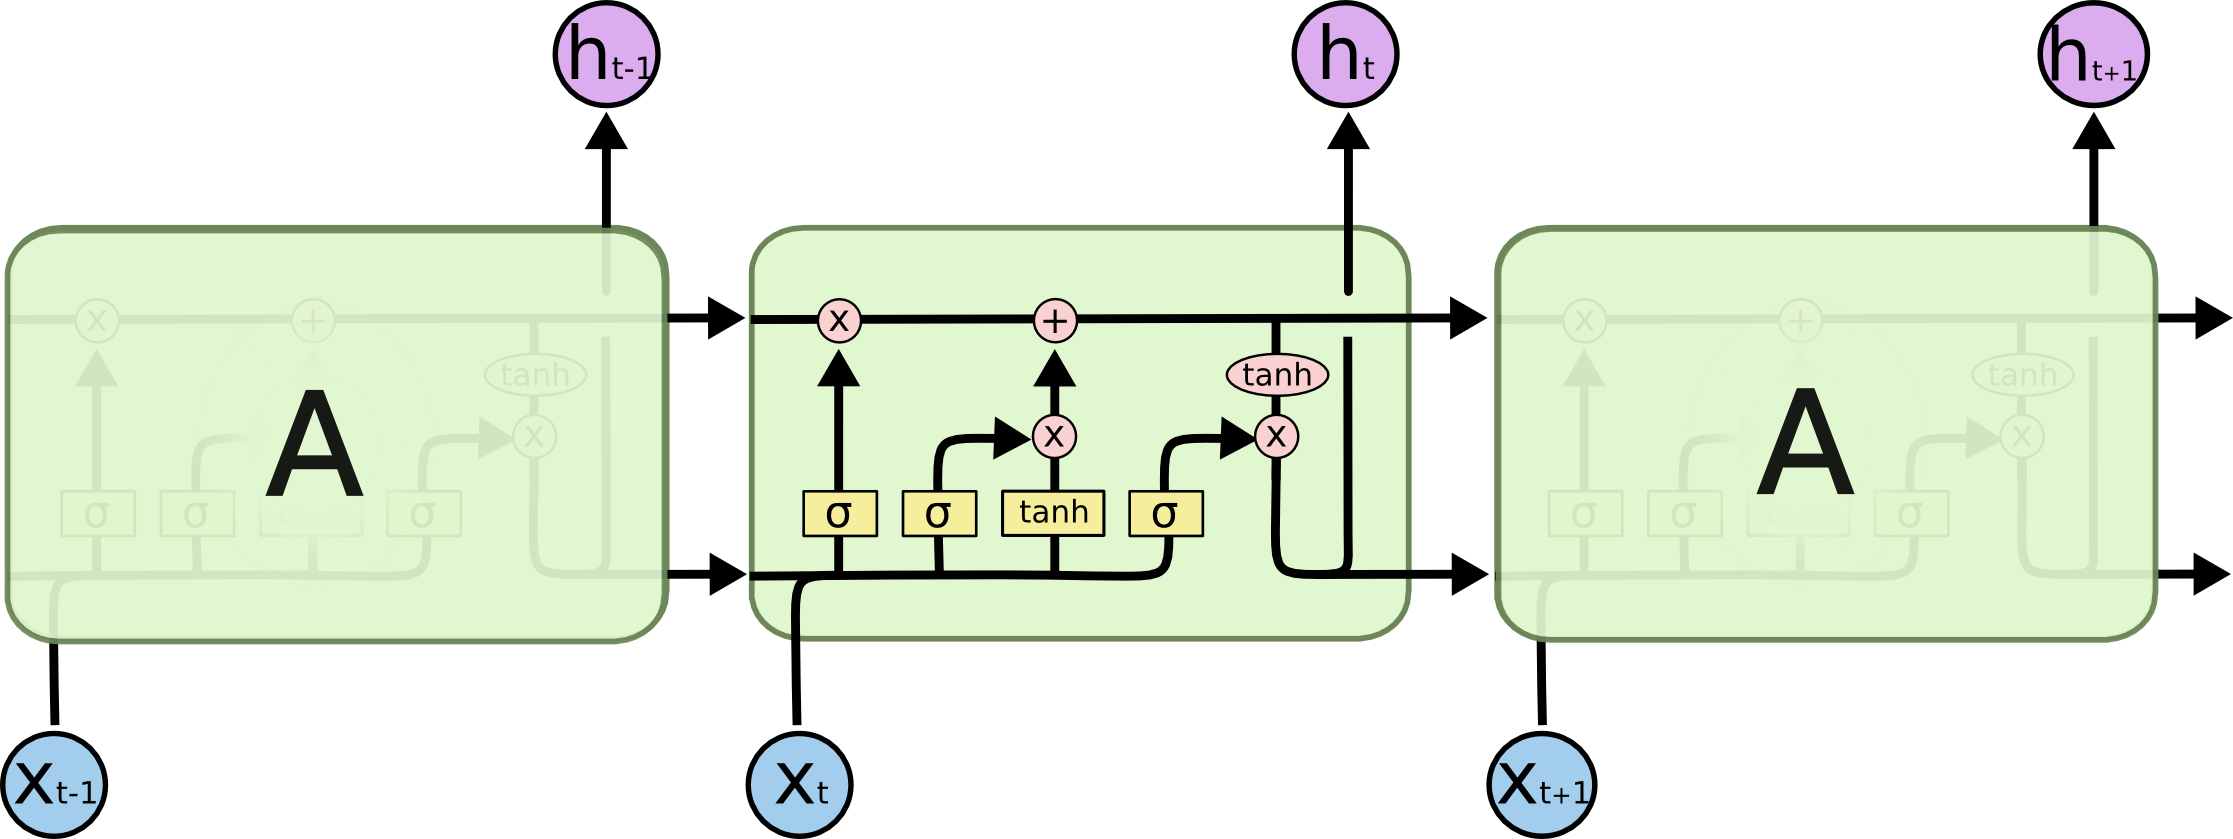
\includegraphics[width=0.90\textwidth]{img/lstm_colah.png}
	\caption{Schemat komórki LSTM. Źródło: http://colah.github.io/posts/2015-08-Understanding-LSTMs/}
	\label{fig:lstm}
\end{figure}


\bibliography{bibliography}

\tableofcontents

\listoffigures

\end{document}